\documentclass[
 size=12pt,
 paper=smartboard, %a4paper, smartboard, screen
 mode=present, %present, handout, print
 display=slides, % slidesnotes, notes, slides
 style=tuliplab,  % TULIP Lab style
 pauseslide,
 fleqn,leqno,clock]{powerdot}

\usepackage{amssymb}
\usepackage{amsmath}
\usepackage{rotating}
\usepackage{graphicx}
\usepackage{boxedminipage}
\usepackage{media9}
\usepackage{rotate}
\usepackage{calc}
\usepackage[absolute]{textpos}
\usepackage{psfrag,overpic}
\usepackage{fouriernc}
\usepackage{pstricks,pst-node,pst-text,pst-3d,pst-grad}
\usepackage{moreverb,epsfig,color,subfigure}
\usepackage{color}
\usepackage{pstricks}
\usepackage{pstricks-add}
\usepackage{pst-text}
\usepackage{pst-node, pst-tree}
\usepackage{booktabs}
\usepackage{etex}
\usepackage{breqn}
\usepackage{multirow}
% \usepackage{pst-rel-points}
\usepackage{listings}
\usepackage{hyperref}
\hypersetup{ % TODO: PDF meta Data
  pdftitle={Presentation Title},
  pdfauthor={Gang Li},
  pdfpagemode={FullScreen},
  pdfborder={0 0 0}
}


% \usepackage{auto-pst-pdf}
% package to show source code

\definecolor{LightGray}{rgb}{0.9,0.9,0.9}
\newlength{\pixel}\setlength\pixel{0.000714285714\slidewidth}
\setlength{\TPHorizModule}{\slidewidth}
\setlength{\TPVertModule}{\slideheight}
\newcommand\highlight[1]{\fbox{#1}}
\newcommand\icite[1]{{\footnotesize [#1]}}

\newcommand\twotonebox[2]{\fcolorbox{pdcolor2}{pdcolor2}{#1\vphantom{#2}}\fcolorbox{pdcolor2}{white}{#2\vphantom{#1}}}
\newcommand\twotoneboxo[2]{\fcolorbox{pdcolor2}{pdcolor2}{#1}\fcolorbox{pdcolor2}{white}{#2}}
\newcommand\vpspace[1]{\vphantom{\vspace{#1}}}
\newcommand\hpspace[1]{\hphantom{\hspace{#1}}}
\newcommand\COMMENT[1]{}

\newcommand\placepos[3]{\hbox to\z@{\kern#1
        \raisebox{-#2}[\z@][\z@]{#3}\hss}\ignorespaces}


%%%%%%%%%%%%%%%%%%%%%%%%%%%%%%%%%%%%%%%%%%%%%%%%%%%%%%%%%%%%%%%%%%%%%%%%%%
%%% title
%%% TODO: Customize to your Own Title, Name, Address
%%%
\title{FLIP(00) Mid-term Presentation}
\author{Rongxin Xu\\
Hunan University
% \href{mailto:gangli@acm.org}{gangli@acm.org}
% \and % more authors
}
\date{26 October 2019}



% Customize the setting of slides
\pdsetup{
% TODO: Customize the left footer, and right footer
rf={\copyright \emph{FLIP(00)}},
cf={FLIP(00) Presentation },
}


% Starts the document
\begin{document}

\maketitle

%%==========================================================================================
%%
\begin{slide}[toc=,bm=]{Outline}
  \tableofcontents[content=sections]
\end{slide}
%%
%%==========================================================================================

\section{Problem Statement}

\begin{slide}{Problem Description}
	\begin{center}
		    This is a problem with time-series prediction.
			After a month of making scientific observations
			and taking careful measurements,
			can predict total sales for every product and store in the next 
			month.
			The raw dataset contains  train set with 2935849
				samples and 214200 unlabeled samples as test set.
			Through the train data, predict total sales for every 
			product and
				store in the next month.
	\end{center}
\end{slide}

\begin{slide}{Data Set}
	\begin{center}
		\twotonebox{\rotatebox{90}{Defn}}{\parbox{.96\textwidth}
			{There are 6 data sets with a total of 11 attributes,
				the fllowings are the
				name and meaning of attributes.
		}}
	\end{center}
	\begin{center}
		\begin{itemize}
			\item Data List
		\end{itemize}
		\begin{description}
			\item[id]  an Id that represents a (Shop, Item) tuple within the 
			test set.
			\item[shop\_id] unique identifier of a shop.
			\item[item\_id] unique identifier of a product.
			\item[item\_category\_id] unique identifier of item category.
			\item[item\_cnt\_day] percentage of soul in the creature.
			\item[item\_price] current price of an item.
			\item[date] date in format dd/mm/yyyy.
			\item[date\_block\_num] unique identifier of item category.
			\item[item\_name] name of item.
			\item[shop\_name] name of shop.
			\item[item\_category\_name] name of item category.
		\end{description}
	\end{center}
\end{slide}

\section{Exploratory Data Analysis}
%
\begin{slide}{Data Information}
 	\begin{center}
 	The following 	is the statistical 
 	result of each attribute in sales\_train.csv.
 	There are 6 numerical variables,
 	and no missing values.
 	The data is very clean and complete, So let's start visual
 	analysis.
 \end{center}
 	\begin{tabular}{ccccccc}
 		\hline
 		% after \\: \hline or \cline{col1-col2} \cline{col3-col4} ...
 		& date\_block\_num   & shop\_id & item\_id & item\_price &
 		item\_cnt\_day
 		& 
 		item\_category\_id                                                      
 		   \\
 		\hline
 		count & 2935849            & 2935849  & 2935849  & 2935849     & 
 		2935849 & 2935849 \\
 		mean  & 14.57              & 33       & 10197.23 & 890.62      & 
 		1.24    & 40      \\
 		std   & 9.42               & 16.23    & 6324.3   & 1726.44     & 
 		2.62    & 17.1    \\
 		min   & 0                  & 0        & 0        & -1          & 
 		-22     & 0       \\
 		25\%  & 7                  & 22       & 4476     & 249         & 
 		1       & 28      \\
 		50\%  & 14                 & 31       & 9343     & 399         & 
 		1       & 40      \\
 		75\%  & 23                 & 47       & 15684    & 999         & 
 		1       & 55      \\
 		max   & 33                 & 59       & 22169    & 307980      & 
 		2169    & 83      \\
 		\hline
 		%\bottomrule
 	\end{tabular}
\end{slide}

\begin{slide}{Data Visualization}
	\begin{center}
	\twotonebox{\rotatebox{90}{Exp}}{\parbox{.96\textwidth}
		{Use EDA to plot the distribution of the data,
			can observate the data intuitively and
			find the relation between the attribute values.
	}}
\end{center}
\begin{center}
	\begin{itemize}
		\item Figures
		\begin{itemize}
			\item Histogrm
			\item Boxplot
			\item Scatterplot Plot
			\item Correllogram
		\end{itemize}
	\end{itemize}
\end{center}
\end{slide}

\begin{slide}{Data Visualization}
	\begin{center}
	\twotonebox{\rotatebox{90}{Exp}}{\parbox{.96\textwidth}
		{It seems that item\_id and
			shop\_id has a huge impact on sales and sales tend to decline
			with the date.
	}}
\end{center}

\begin{center}
	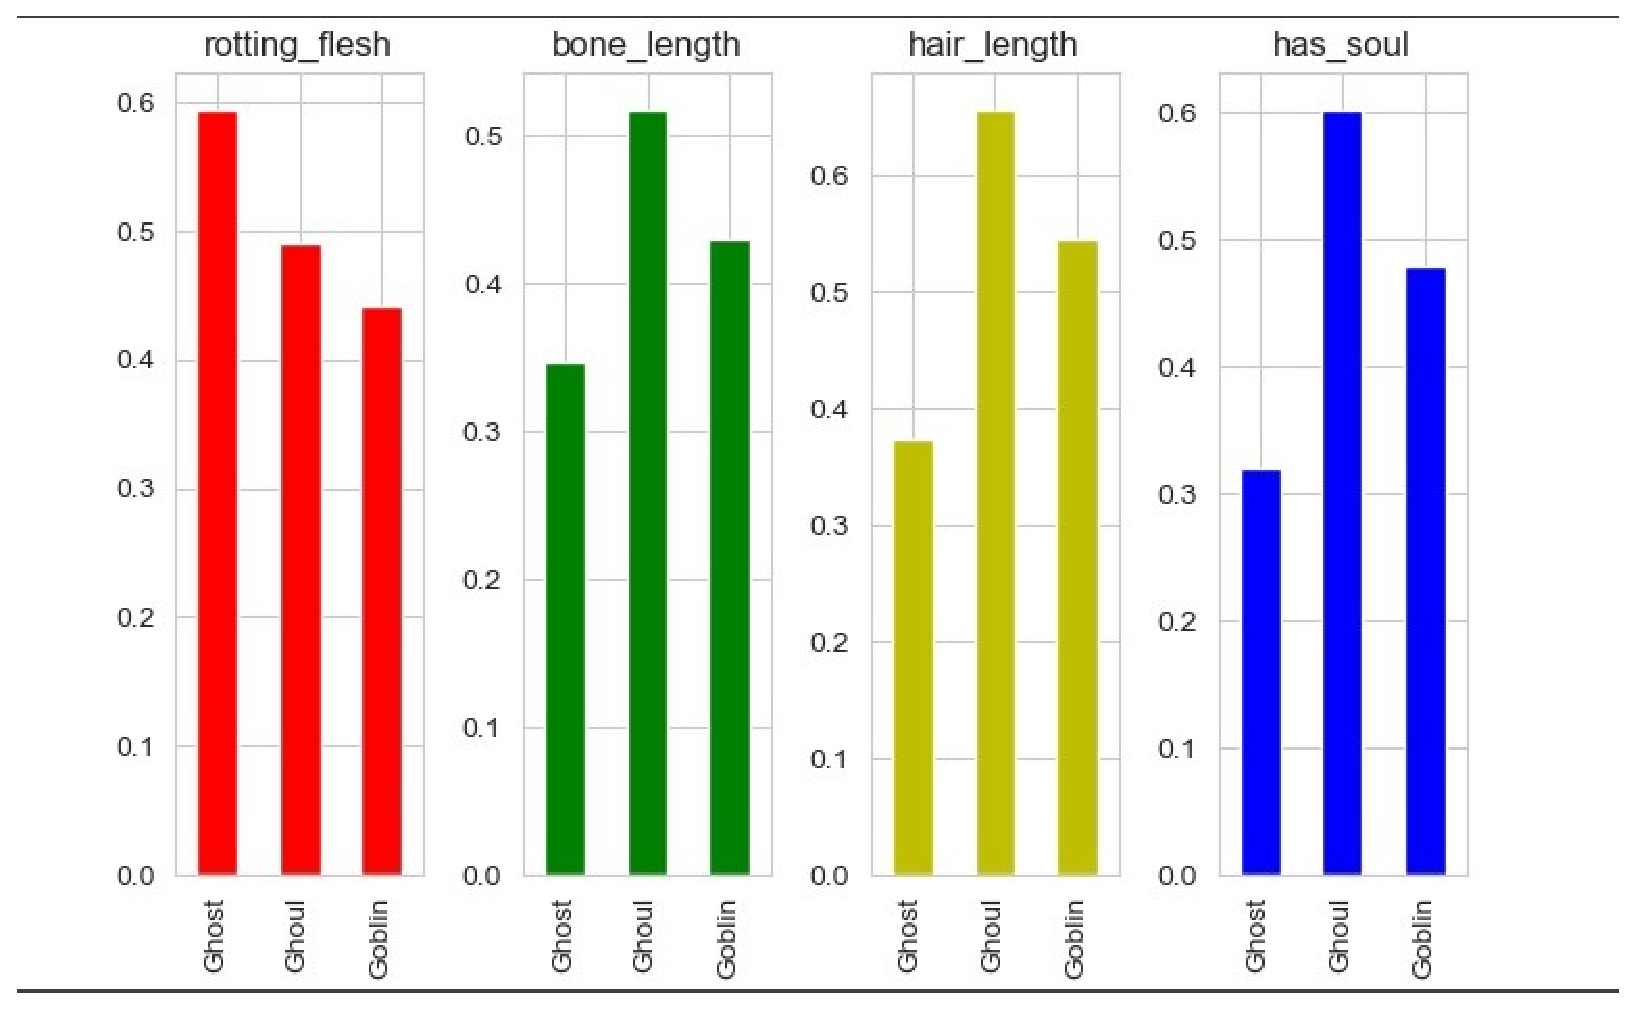
\includegraphics[width=.4\linewidth,height=.4\linewidth]{figures/his_1.eps}
	\quad\includegraphics[width=.4\linewidth,height=.4\linewidth]{figures/his_2.eps}
\end{center}
\end{slide}

\section{Data Visualization}

\begin{slide}{Exploratory Data Analysis}
	\begin{center}
	\twotonebox{\rotatebox{90}{Exp}}{\parbox{.96\textwidth}
		{When analyzing the data,
			the boxplot can effectively
			help us identify the characteristics of the data:
			visually identify outliers in the dataset or
			determine the data dispersion and
			bias of the data set.
			We can see that the outliers are very small,
			so can be ignored.
	}}
\end{center}

\begin{center}
	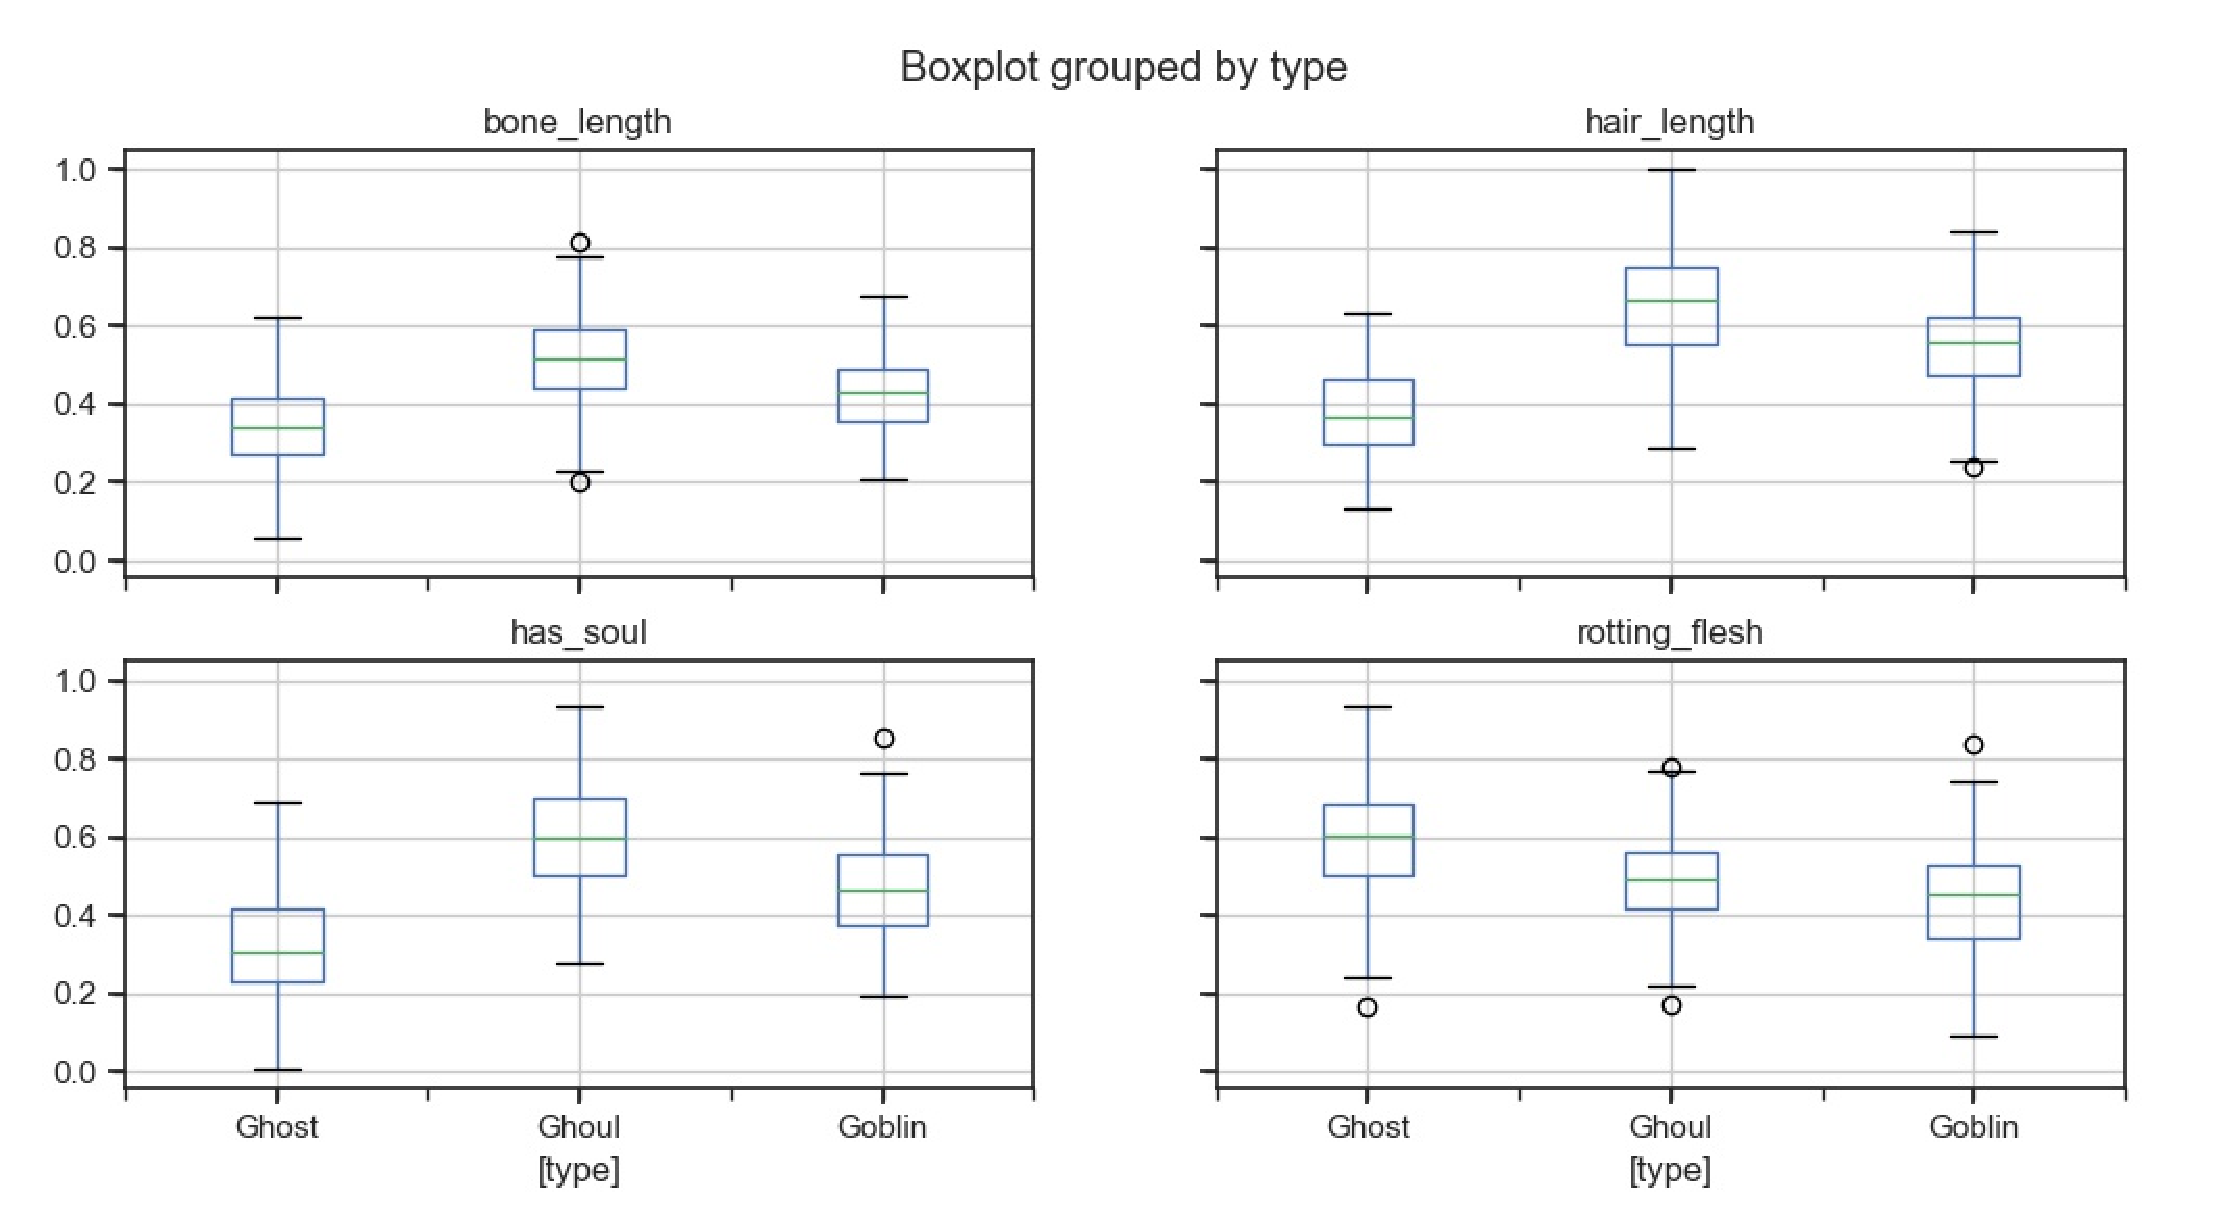
\includegraphics[width=.4\linewidth,height=.4\linewidth]{figures/boxplot.eps}
	\quad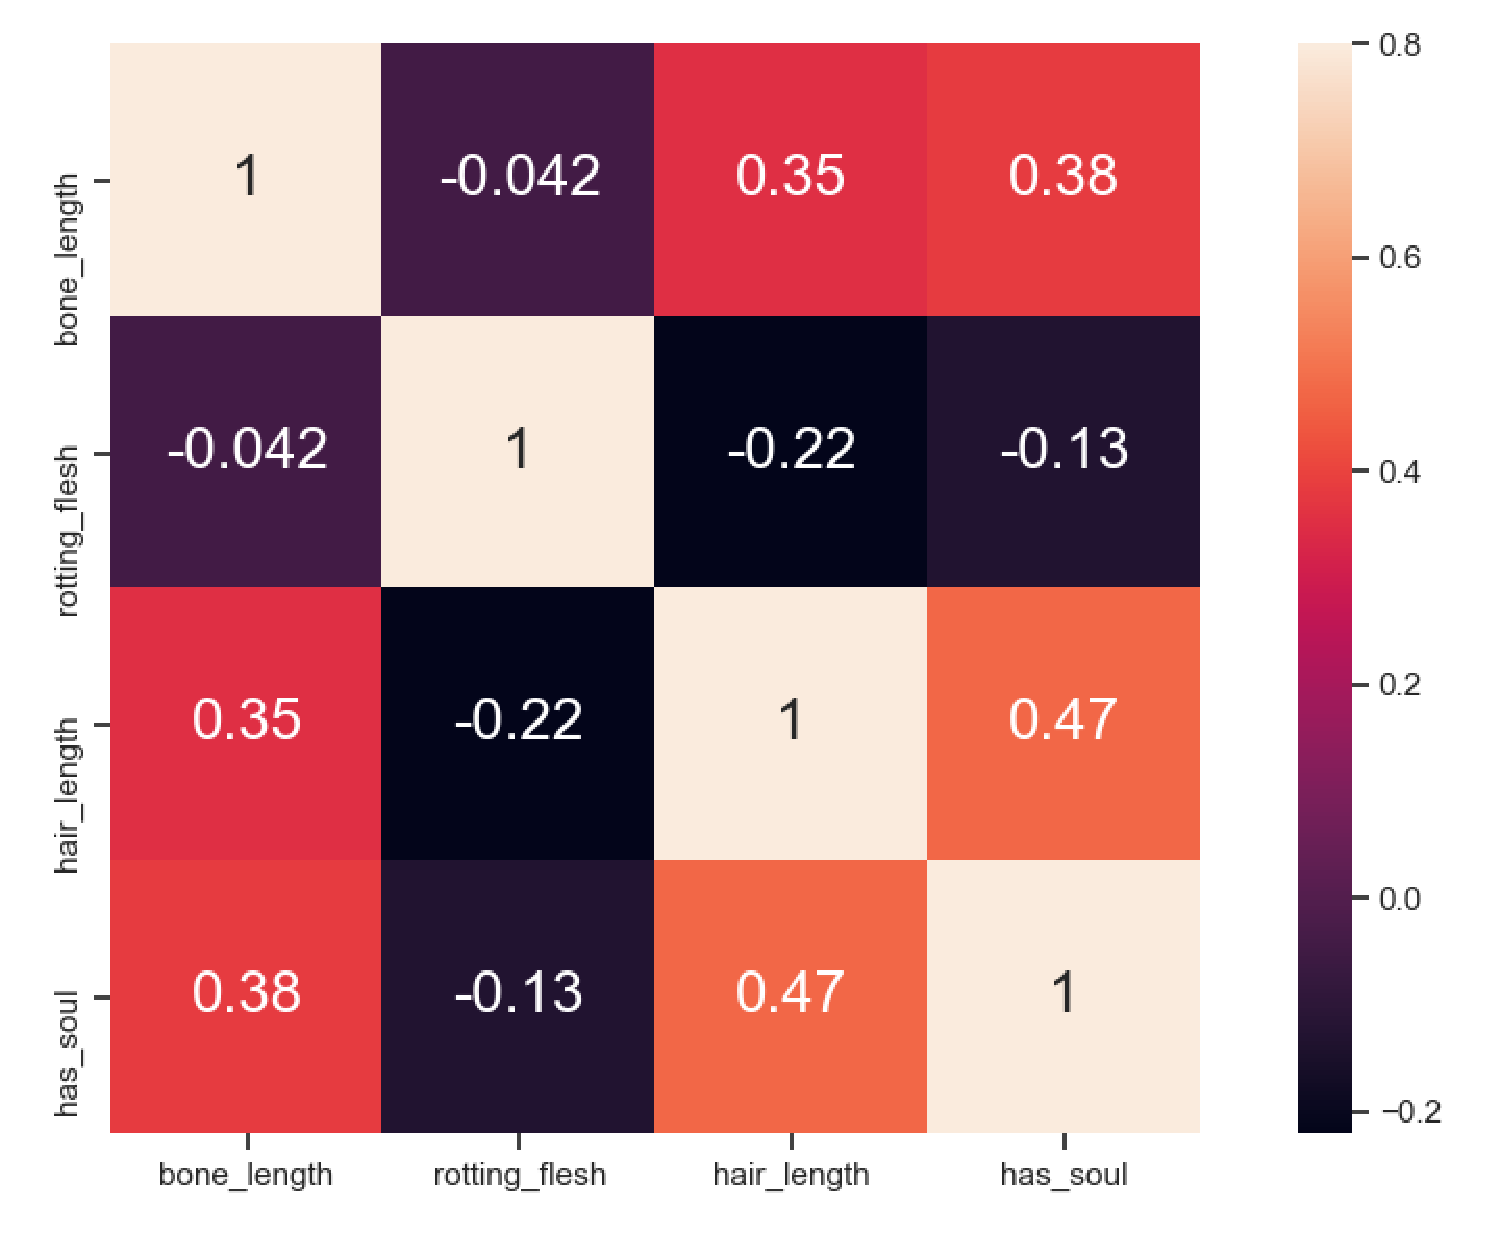
\includegraphics[width=.4\linewidth,height=.4\linewidth]{figures/corr.eps}
\end{center}
\end{slide}

\begin{slide}{Summary}
  \begin{itemize}
    \item
          There is an obvious "seasonality" (Eg: peak sales around a time of year)
          and a decreasing "Trend".
  \end{itemize}
\end{slide}

\section{Stationarity}

\begin{slide}{Seasonality and Trend}
  \begin{figure}
    \centering
    % Requires \usepackage{graphicx}
    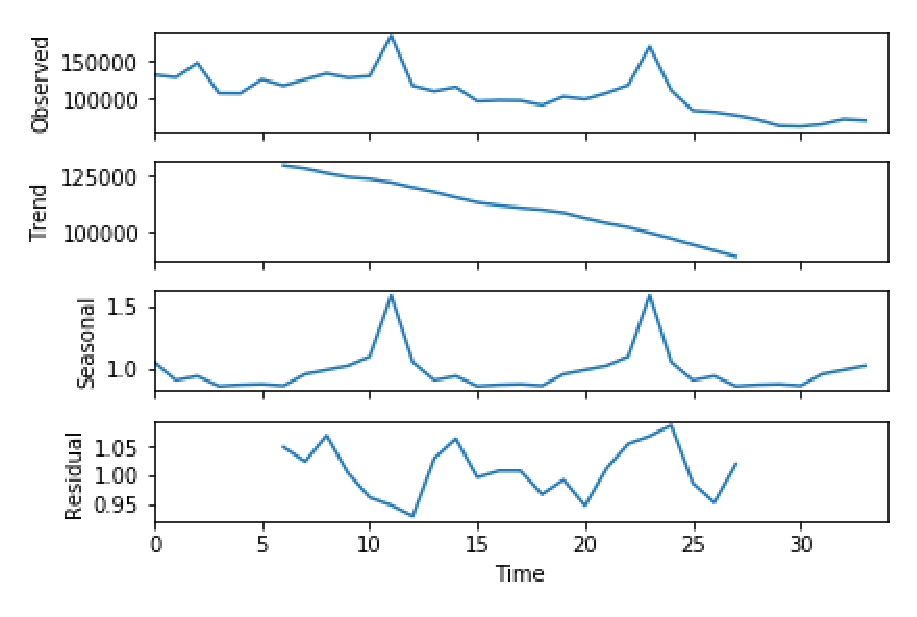
\includegraphics[width=5in]{Figures/9.eps}
    \caption{Seasonality and Trend}
    \label{Seasonality and Trend}
  \end{figure}
\end{slide}

\begin{slide}{Stationarity Test}
  \begin{figure}
    \centering
    % Requires \usepackage{graphicx}
    \includegraphics[width=4in]{Figures/10.eps}
    \caption{Stationarity Test}
    \label{Stationarity Test}
  \end{figure}
\end{slide}

\begin{slide}{Remove seasonality and trends}
  \begin{figure}
    \centering
    % Requires \usepackage{graphicx}
    \includegraphics[width=6in,height=4in]{Figures/11.eps}
    \caption{Remove seasonality and trends}
    \label{Remove seasonality and trends}
  \end{figure}
\end{slide}

\begin{slide}{Summary}
  \begin{itemize}
    \item
          Now let's check the new P-value.
          \begin{figure}
            \centering
            % Requires \usepackage{graphicx}
            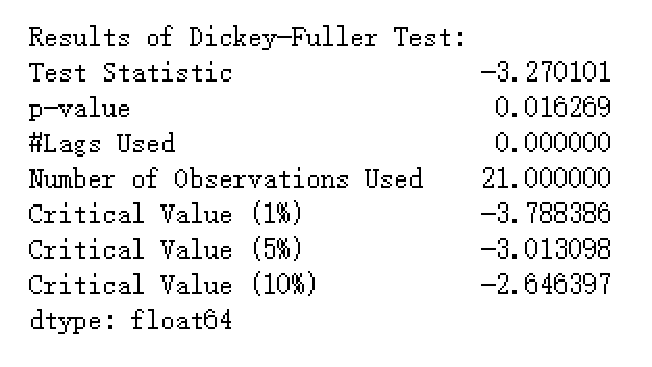
\includegraphics[width=3in,height=2in]{Figures/12.eps}
            \caption{new stationarity test}
            \label{new stationarity test}
          \end{figure}
    \item
          After the transformations, our p-value for the DF test is well within 0.05.
          Hence we can assume Stationarity of the series.
  \end{itemize}
\end{slide}

\section{Conclusion}
\begin{slide}{Summary}
  \begin{itemize}
    \item From the above result presentation, we can find that
          \subitem There are seasonality and trend in data.
          \bigskip
    \item From the Stationarity test, we can find that
          \subitem After removing seasonality and trends, the time series becomes smooth.
          \smallskip
          \subitem So we can use traditional time series prediction methods for prediction.
  \end{itemize}
\end{slide}

\begin{slide}{Future research}
  \begin{itemize}
    \item Predict by traditional time series prediction models such as AR, MA and ARMA.
    \item Using more models to predict, such as random forests and neural networks.
    \item Find the most effective model and get my own kaggle ranking.
  \end{itemize}
\end{slide}

\begin{wideslide}[toc=,bm=]{}
  \centering
  \vspace{\stretch{1}}
  \twocolumn[
    lcolwidth=0.35\linewidth,
    rcolwidth=0.65\linewidth
  ]
  {
    % \centerline{\includegraphics[scale=.2]{tulip-logo.eps}}
  }
  {
    \vspace{\stretch{1}}


    \textcolor{black}{\scalebox{2.0}{Thank you \& Question}}


  }
  \vspace{\stretch{1}}
\end{wideslide}

\end{document}
\endinput
